\section{Asure Network}

The Asure protocol builds upon three components.

\begin{itemize}
\item \textbf{Scaled Blockchain Network:} We provide an abstraction for network of independent providers to offer application services. Later, we present the Asure protocol as an incentivized, auditable and verifiable construction.
\item \textbf{Platform:} By providing a platform that enables the development of social security systems on top of blockchain technologies.
\item \textbf{Protocol:} Social security systems exist in many different forms and Asure is providing general design specifications on how to implement these applications on blockchain.
halölo

\end{itemize}

\begin{figure}
    \centering
    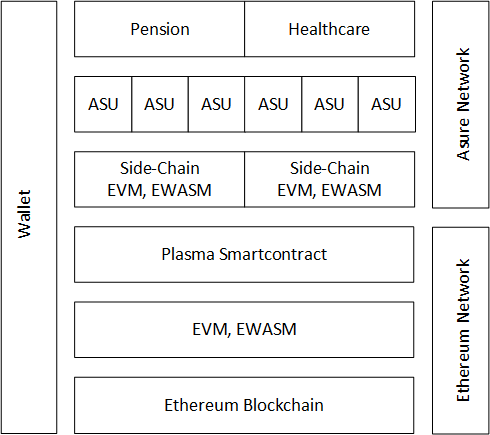
\includegraphics[width=4.0in]{architecture.png}
    \caption{Asure architecture}
    \label{fig:asure_architecture}
\end{figure}

\subsection{Plasma}

Plasma is a framework. Plasma was very recently introduced and is among the more promising proposed solutions to scalable computation on the blockchain. Plasma can provide real scalability for ethereum applications. 
\newline
Plasma is an application-specific sidechain protocol.

Although the proposed Layer 2 protocols are still at an early stage and have not been described in detail, they essentially work by sending transactions to an off-chain platform. 

In order to raise the limits of layer 1 even further in order to effectively operate the social security system user group, layer-2 scaling is considered to be the most likely solution. Plasma is a good approach to the challenges of most.

\subsection{Sidechain}

Your chain will connect to Ethereum, inheriting its security and accountability. Your chain will be a sidechain.
\newline
This setup is the best of both worlds: From one part, it frees you from having to deal with securing your chain. For that, you can depend on the layer 1 chain.
\newline
From the other side, you can design your sidechain to match your needs.


\begin{figure}
    \centering
    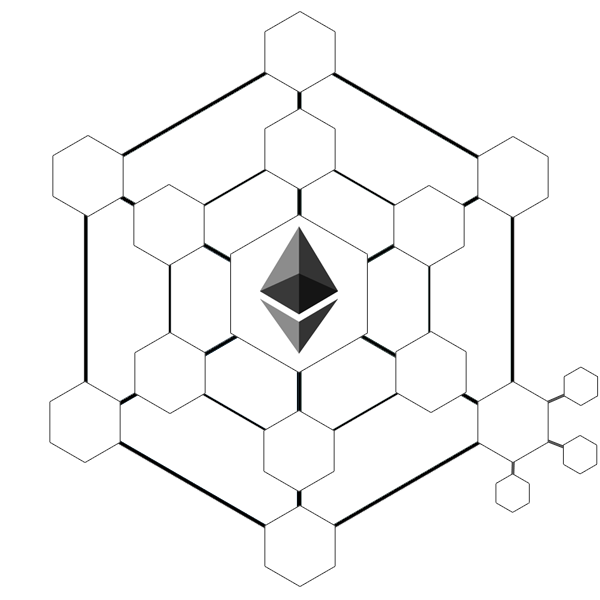
\includegraphics[width=4.0in]{side-chain.png}
    \caption{Asure side chains}
    \label{fig:side_chain}
\end{figure}

\subsection{Protocol}

Plasma is not an implementation. It’s a protocol, or a set of guidelines. As long as you follow the specifications, your sidechain will be plasma.

\subsection{Plasma + EVM}

EVM provides such a powerful turing-complete computation so that ethereum can run a general program, also known as smart contract. Plasma EVM is a new version of Plasma that can execute EVM in plasma chain, and its clients can be based on current ethereum clients (go-ethereum, py-evm, parity). We propose state-enforceable Plasma construction to guarantee only valid state submitted to root chain, providing a way to enter and exit account storage between two chains because each chain has identical architecture. Another benefit is that ethereum development tools can be also used in plasma chain.

\subsection{Plasma + WASM, eWASM, *WASM}

WASM seems more secure, webassembly is backed by Google, Apple and Microsoft, the community is also active, it's gonna be a widely used platform. 
So embrace WASM will be a really good choice.

eWASM is a restricted subset of WASM (WebAssembly) to be used for contracts in Ethereum.